\documentclass[pdf,hyperref={unicode}]{beamer}

\usetheme{Berlin}
\usepackage[utf8]{inputenc}
\usepackage[czech]{babel}
\usepackage{graphicx}
\usefonttheme{professionalfonts}

\date{}
\setbeamertemplate{headline}{}
\setbeamertemplate{navigation symbols}{}
\setbeamertemplate{footline}
{

 \hbox{%
  \begin{beamercolorbox}[wd=.11111\paperwidth,ht=2.25ex,dp=1ex,center]{author in head/foot}%
  \usebeamerfont{author in head/foot} VUT FIT
  \end{beamercolorbox}%

   \begin{beamercolorbox}[wd=.77777\paperwidth,ht=2.25ex,dp=1ex,center]{title in head/foot}%
    
   \usebeamerfont{author in head/foot} Martin Vlach, Lukáš Hekrdla, Martin J. Salamánek, Tomáš Tlapák
    \end{beamercolorbox}%

  \begin{beamercolorbox}[wd=.11111\paperwidth,ht=2.25ex,dp=1ex,center]{date in head/foot}%
    \insertframenumber{} / \inserttotalframenumber 
  \end{beamercolorbox}}%
  \vskip0pt% 
}

\title{Překladač imperativního jazyka IFJ2018}
\author{Tým 087 varianta I}
\institute[VUT FIT]
{
	{\large Vysoké učení technické v Brně} \\[0,4em]
    {\large Fakulta informačních technologií}
} 


\begin{document}

\begin{frame}
	\titlepage
\end{frame}

\begin{frame}
\frametitle{Struktura překladače}
\hspace*{-4ex}\includegraphics[scale=0.4]{schema.eps}
\end{frame}


\begin{frame}
\frametitle{Práce v týmu}
	\begin{center}
	\begin{itemize}
	\item používání verzovacího systému Git
	\item využívání  některých prvků extrémního programování
		\begin{itemize}
			\item párové programování
			\item společné vlastnictví kódu
			\item atd\,\dots
		\end{itemize}
	\end{itemize}
	\end{center}
\end{frame}

\begin{frame}
\frametitle{Testování}
	\begin{itemize}
		\item dynamické testování
		\item modulární testování
		\item manuální testování 
	\end{itemize}
\end{frame}

\begin{frame}
\frametitle{Abstraktní datové typy}
	\begin{itemize}
		\item binární vyhledávací strom
		 	\begin{itemize}
		 	 \item binární vkládání a hledání
		 	 \item $O(log_2 \ n)$ průměrná náročnost
		 	 \item $O(n) $ nejhorší náročnost 
		 	\end{itemize}
		 \item další použité struktury:
		  \begin{itemize}
		  \item  jednosměrně vázaný seznam
		  \item zásobník
		\end{itemize}		 
	\end{itemize}
\end{frame}


\begin{frame}
\begin{center}
{\huge Děkujeme za pozornost \\[15px] Prostor pro dotazy\,\dots}
\end{center}
\end{frame}


\end{document}